\documentclass[final,xcolor=dvipsnames]{beamer}
%
% Choose how your presentation looks.
%
% For more themes, color themes and font themes, see: 
% http://deic.uab.es/~iblanes/beamer_gallery/index_by_theme.html
%

%the-sun-is-in-love-with-the-moon-collab-with-blaak.jpg

\mode<presentation>
{
  \usetheme{Boadilla}      % or try Darmstadt, Madrid, Warsaw, ...
  \usecolortheme{default} % or try albatross, beaver, crane, ...
  \usefonttheme{structurebold}  % or try serif, structurebold, ...
  \setbeamertemplate{navigation symbols}{}
  \setbeamertemplate{caption}[numbered]
} 

\usepackage[english]{babel}
\usepackage[utf8x]{inputenc}
\usepackage[]{caption}
\usepackage{tikz}

\usepackage{phaistos}

%% Section name as title %%% 
%\addtobeamertemplate{frametitle}{\let\insertframetitle\insertsubsectionhead}{}
%\addtobeamertemplate{frametitle}{\let\insertframesubtitle\insertsectionhead}{}
%\makeatletter
%  \CheckCommand*\beamer@checkframetitle{\@ifnextchar\bgroup\beamer@inlineframetitle{}}
%  \renewcommand*\beamer@checkframetitle{\global\let\beamer@frametitle\relax\@ifnextchar\bgroup\beamer@inlineframetitle{}}
%\makeatother
%% %% %% %% 

%\titlegraphic{\includegraphics[]{the-sun-is-in-love-with-the-moon-collab-with-blaak.jpg} \hspace{2cm} \includegraphics[width=2cm]}}
\title[Introduction to Environmental Modelling]{Introduction to Environmental Modelling}
\subtitle{Face-It Summer School 2019 : Marine Biogeochemical Cycling: from measurements to modelling}
\author[A. Capet]{A. Capet, M.Grégoire, K. Soetaert} %Logo de MAST +logo interface sur chaque slide et page de garde interface?
\institute[http://labos.ulg.ac.be/mast/]{MAST - acapet@ulg.ac.be}
\date[Oct 2019]

%\AtBeginSubsection[]{
%  \begin{frame}
%  \vfill
%  \centering
%  \begin{beamercolorbox}[sep=8pt,center,shadow=true,rounded=true]{title}
%    \usebeamerfont{title}\insertsectionhead\par%
%    \usebeamerfont{title}\insertsubsectionhead\par%
%  \end{beamercolorbox}
%  \vfill
%  \end{frame}
%}

\AtBeginSubsection[]{
  \frame<beamer>{ 
    \frametitle{Outline}   
    \tableofcontents[currentsection,currentsubsection] 
  }
}

\begin{document}
\def\mussel{\PHoxBack}
\def\extitle[#1]{\centering{ \mussel \hspace{2cm} #1 \hspace{2cm} \mussel}}
% \usebackgroundtemplate{%             declare it
% \tikz[overlay,remember picture] \node[opacity=0.6, at=(current page.center)] {
%   \includegraphics[height=\paperheight,width=\paperwidth]{the-sun-is-in-love-with-the-moon-collab-with-blaak.jpg}
%   };
%   % {Great_Barrier_Reef_Australia}};
% }

\begin{frame}
  \titlepage
\end{frame}

% \usebackgroundtemplate{ }  

\section{Basics Concepts}
\subsection{What is a model ?}
\begin{frame}
\visible<2>{
 A \alert{simplified} representation of a complex phenomenon.} 
\end{frame}

\begin{frame}{How simple ?}
\centering{Arguments in favor of:}
\begin{columns}
\begin{column}{.5\framewidth}
\centering{\alert{Simplicity}}
\end{column}
\begin{column}{.5\framewidth}
\centering{\alert{Complexity}}
\end{column}
\end{columns}
\end{frame}


\section{Elements of a model}
\subsection{Research Questions}

\begin{frame}
\begin{block}{Research Questions}
\begin{itemize}
    \item Clear formulation of the research question should lead decisions for all elements of the model 
\end{itemize}
\end{block}
\end{frame}

\begin{frame}
\begin{exampleblock}{\extitle[Research Context]}
\begin{columns}
\begin{column}{0.5\framewidth}
\begin{figure}
    \centering
    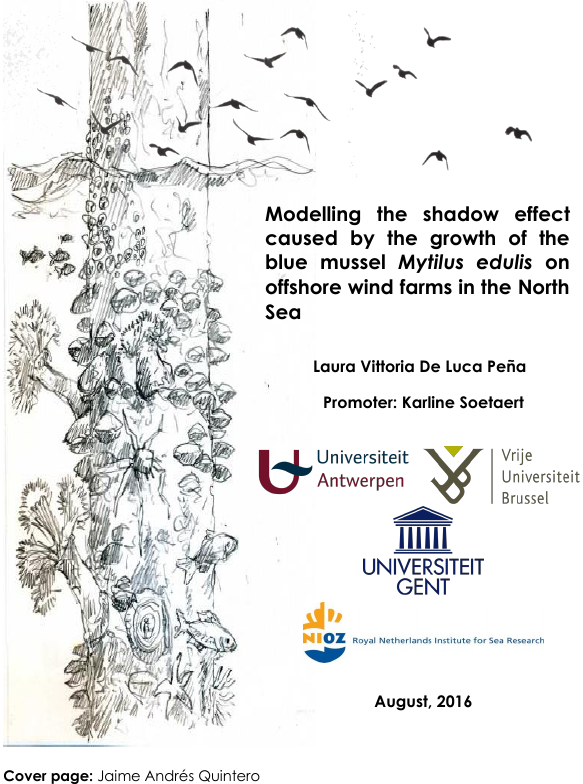
\includegraphics{./Figs/Context.png}
    \caption{Caption}
    \label{fig:my_label}
\end{figure}
\end{column}
\begin{column}{0.5\framewidth}
Our study mainly focuses on 
\begin{itemize}
    \item increased production of organic matter (faeces and pseudofaeces)
    \item food depletion by the growth of biofouling %organisms
    \item impacts on biogeochemical processes via respiration and excretion. 
\end{itemize}
\end{column}
\end{columns}
\end{exampleblock}
\end{frame}

\begin{frame}
\begin{exampleblock}{\extitle[Research Questions]}
\begin{itemize}
    \item How deep can the blue mussels grow under mixed/stratified conditions,
    \item Will there be local depletion of food resources such as phytoplankton, zooplankton and detritus ?
    \item Will mussels on seabed have the same effect as mussel on the structure ? 
    \item Does type of turbine and distance between them impacts on the accumulation of mussel biomass and on ecosystem and biogeochemical dynamics ?
\end{itemize}
\end{exampleblock}
\end{frame}

\subsection{Scales}
\begin{frame}
\begin{block}{Spatial Scales}
\begin{itemize}[<+->]
    \item Relevant scales for system dynamics ?
    \item Relevant scale for operating processes ?
    \item Non-linearities ?
    \item Anisotropy? In forcings ? in processes ?
    \item Length scale of spatial resolution for available observations ?
    \item Memory ! 
\end{itemize}
\end{block}

\pause

\begin{exampleblock}{\extitle[Spatial Scales]}
\begin{itemize}
    \item 1-dimension
    \item 25 m pylone
    \item 50 layers of 0.5 m each
    \item Horizontal lenght scales
\end{itemize} 
\end{exampleblock}

\end{frame}

\begin{frame}
\begin{block}{Temporal Scales}
\begin{itemize}[<+->]
    \item Relevant scales for system dynamics
    \item Relevant scale for operating processes
    \item Non-linearities
    \item Periodicity in forcings ?  
    \item CPU ! 
\end{itemize}
\end{block}

\end{frame}



\subsection{State Variables}
\begin{frame}
NPZD Approach
Common Currency : Nitrogen
\begin{exampleblock}{State variables}
\begin{itemize}
    \item ammonium (NH4),
    \item nitrate (NO3),
    \item phytoplankton (PHYTO)
    \item zooplankton (ZOO)
    \item detritus (PELDETRITUS),
    \item bottom detritus (BOTDETRITUS)
\end{itemize} 
\end{exampleblock}

\begin{exampleblock}
Two domains of different dimensionality.
\end{exampleblock}
\end{frame}

\subsection{Dynamic Equation}
\begin{frame}
\begin{block}{Mass Blance Equation}
\begin{itemize}
    \item Only N limits phyto growth
    \item Both NH4 and NO3 Uptaken, but NH3 favored (limitation).
    \item Light limits plankton Growth  
    \item Liebig's law of the minimum
    \item Mussels feeds on Phytoplankton
    \item Zooplankton feeds on phytoplankton
\end{itemize} 
\end{block}
\end{frame}


\begin{frame}
\begin{exampleblock}{Assumptions}
\begin{itemize}
    \item Only N limits phyto growth
    \item Both NH4 and NO3 Uptaken, but NH3 favored (limitation).
    \item Light limits plankton Growth  
    \item Liebig's law of the minimum
    \item Mussels feeds on Phytoplankton
    \item Zooplankton feeds on phytoplankton
\end{itemize} 
\end{exampleblock}
\end{frame}

\subsection{Conservation ?}

\subsection{External Inputs}
\begin{frame}

\begin{exampleblock}{Scales}
\begin{itemize}
    \item a one-dimensional k-$\epsilon$ turbulence closure model 
    \item Temperature
    \item Current Velocity
    \item Turbulent Kinetic Energy
    \item (Salinity Constant)
\end{itemize} 
\end{exampleblock}
\end{frame}



\section{Integration}
\begin{frame}{Frame Title}
    
\end{frame}


\section{Model VS Real World}


\subsection{Error Observations}
\begin{frame}{Frame Title}
    

* Difficulty in confronting discrete sampling with model continuous observations. 
* Match the definition of state variables.

\begin{exampleblock}{Observations}
\begin{itemize}
    \item Nutrients (upwind, downwind)
    \item Phytoplankton (which proxy)
    \item Sediment content (heterogeneity)
    \item .. 
\end{itemize} 
\end{exampleblock}
\end{frame}


\end{document}

